\documentclass{standalone}
\usepackage{pgfplots}
\pgfplotsset{compat=1.18}
\usepgfplotslibrary{colorbrewer}
\pgfplotsset{cycle list/Set1-6}

\begin{document}

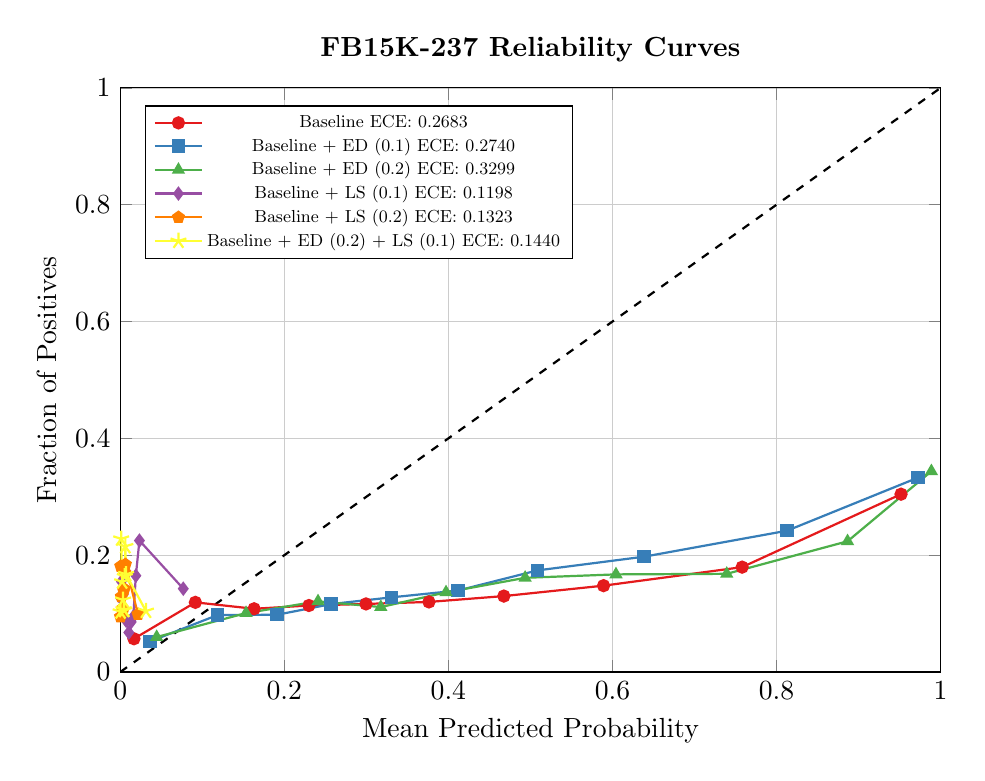
\begin{tikzpicture}
\begin{axis}[
    title={\textbf{FB15K-237 Reliability Curves}},
    xlabel={Mean Predicted Probability},
    ylabel={Fraction of Positives},
    xmin=0, xmax=1,
    ymin=0, ymax=1,
    xtick={0, 0.2, 0.4, 0.6, 0.8, 1.0},
    ytick={0, 0.2, 0.4, 0.6, 0.8, 1.0},
    legend pos=north west,
    legend style={nodes={scale=0.7, transform shape}, font=\small},
    grid=both,
    grid style={line width=.1pt, draw=gray!20},
    major grid style={line width=.2pt, draw=gray!40},
    width=12cm,
    height=9cm,
    cycle list name=Set1-6
]

% Perfectly Calibrated Line
\addplot [color=black, dashed, line width=0.8pt, forget plot]
    coordinates {(0,0)(1,1)};
% this is the results for the top 10 hits on the Same method fo the evaluation
% Model 1: Baseline
\addplot+[mark=*, thick] coordinates {
    (0.01665992, 0.05691255) (0.09155014, 0.11922795) (0.16314528, 0.10823357) (0.22998002, 0.11385292) 
    (0.29957646, 0.11654043) (0.37629238, 0.11996091) (0.46759567, 0.12997801) (0.58913222, 0.14781334) 
    (0.75807139, 0.17953102) (0.95175962, 0.30442218)
};
\addlegendentry{Baseline ECE: 0.2683}

% Model 2: Baseline + ED (0.1)
\addplot+[mark=square*, thick] coordinates {
    (0.03633441, 0.05227162) (0.11852617, 0.09748351) (0.19114901, 0.09797215) (0.25703005, 0.11629612) 
    (0.33049231, 0.12777914) (0.41162824, 0.13950647) (0.50859455, 0.17395553) (0.63842163, 0.19741021) 
    (0.81277278, 0.24187637) (0.97231538, 0.33268197)
};
\addlegendentry{Baseline + ED (0.1) ECE: 0.2740}

% Model 3: Baseline + ED (0.2)
\addplot+[mark=triangle*, thick] coordinates {
    (0.04440314, 0.05984367) (0.15332946, 0.10090398) (0.24107407, 0.12093819) (0.31759084, 0.1111654) 
    (0.3970972, 0.13633032) (0.49352611, 0.16125092) (0.60428052, 0.16711459) (0.7393058, 0.16809186) 
    (0.8865653, 0.22379673) (0.98876647, 0.34367367)
};
\addlegendentry{Baseline + ED (0.2) ECE: 0.3299}

% Model 4: Baseline + LS (0.1)
\addplot+[mark=diamond*, thick] coordinates {
    (0.0004922, 0.12652662) (0.00136182, 0.15489861) (0.00350409, 0.13242121) (0.00711733, 0.08795505) 
    (0.01043486, 0.06767652) (0.01330828, 0.08575617) (0.01593354, 0.09479599) (0.01899207, 0.16491571) 
    (0.02339561, 0.22501832) (0.07681628, 0.14264778)
};
\addlegendentry{Baseline + LS (0.1) ECE: 0.1198}

% Model 5: Baseline + LS (0.2)
\addplot+[mark=pentagon*, thick] coordinates {
    (0.00026047, 0.09452858) (0.00058063, 0.1810408) (0.0013168, 0.12900073) (0.00226386, 0.10823357) 
    (0.00330721, 0.10579037) (0.00418406, 0.13950647) (0.00483144, 0.14219399) (0.00541067, 0.17029074) 
    (0.00626516, 0.18421696) (0.02161047, 0.09892526)
};
\addlegendentry{Baseline + LS (0.2) ECE: 0.1323}

% Model 6: Baseline + ED (0.2) + LS (0.1)
\addplot+[mark=star, thick, mark size=3pt] coordinates {
    (0.0003858, 0.10307767) (0.00109858, 0.22795016) (0.0022893, 0.15440997) (0.00342556, 0.12338138) 
    (0.00425036, 0.10676765) (0.00491394, 0.10554605) (0.00552733, 0.16344979) (0.00622427, 0.21500122) 
    (0.00712705, 0.16711459) (0.03136405, 0.10429897)
};
\addlegendentry{Baseline + ED (0.2) + LS (0.1) ECE: 0.1440}

\end{axis}
\end{tikzpicture}

\end{document}